% book example for classicthesis.sty
\documentclass[11pt,a5paper,footinclude=true,headinclude=true]{scrbook} % KOMA-Script book
\usepackage[T1]{fontenc}   
\usepackage[linedheaders,parts,pdfspacing]{classicthesis}
\usepackage{amsmath}
\usepackage{amsthm}
\usepackage{graphicx}
\usepackage{caption}
\usepackage{subcaption}
\usepackage{listings}
\usepackage{color}

\definecolor{bgcolor-code}{rgb}{0.95,0.95,0.92}
\definecolor{bgcolor-out}{rgb}{0,0,0}
\definecolor{txtcolor-out}{rgb}{1,1,1}
\definecolor{bgcolor-file}{rgb}{0.92,0.97,0.97}
\definecolor{txtcolor-file}{rgb}{0,0,0}

\lstdefinestyle{c++}{language=C++,
    backgroundcolor=\color{bgcolor-code}, 
    basicstyle=\ttfamily\small,
    keywordstyle=\color{blue}\ttfamily,
    stringstyle=\color{red}\ttfamily,
    commentstyle=\color{green}\ttfamily,
    morecomment=[l][\color{magenta}]{\#},
    breaklines=true, postbreak=\mbox{\textcolor{red}{$\hookrightarrow$}\space}
}

\lstdefinestyle{out}{
    backgroundcolor=\color{bgcolor-out}, 
    basicstyle=\ttfamily\small\color{txtcolor-out}
}

\lstdefinestyle{file}{
    backgroundcolor=\color{bgcolor-file}, 
    basicstyle=\ttfamily\small\color{txtcolor-file}
}

\theoremstyle{definition}
\newtheorem{definition}{Definition}[chapter]
\newcommand{\code}[1]{\mbox{\texttt{#1}}}

\title{The uunet library:\\an overview}

\begin{document}
%	\pagestyle{scrheadings}
%	\manualmark
%	\markboth{\spacedlowsmallcaps{\contentsname}}{\spacedlowsmallcaps{\contentsname}}
	
	\maketitle
	
	\tableofcontents 

%	\automark[section]{chapter}
%	\renewcommand{\chaptermark}[1]{\markboth{\spacedlowsmallcaps{#1}}{\spacedlowsmallcaps{#1}}}
%	\renewcommand{\sectionmark}[1]{\markright{\thesection\enspace\spacedlowsmallcaps{#1}}}

\cleardoublepage

\chapter{Introduction}

This document provides an overview of the \code{uunet} library, with examples on how to use its classes and functions. It is not aimed at explaining how the algorithms work; references where to learn more about multilayer network theory and methods are available in Chapter \ref{ch:readings}.

The \code{uunet} library contains code used or developed at the Uppsala University Information Laboratory (InfoLab) to store, manipulate and analyze data about interconnected entities. Most of the functions provided by our multilayer network analysis libraries for R\footnote{https://cran.r-project.org/web/packages/multinet/index.html} and Python\footnote{https://pypi.org/project/uunet/} are implemented in \code{uunet}.

While \code{uunet} provides some graph management functionality, it is not intended as a full-fledged graph analysis library; several are already available. \code{uunet} focuses on more expressive data structures, such as multilayer networks.


\section{A short history of the library}

In 2011 we published our first paper on multilayer networks, where we introduced what at the time we called the ML-Model: 
\begin{quote}
Matteo Magnani and Luca Rossi (2011). The ML-Model for Multi-Layer Social Networks. International conference on social network analysis and mining (ASONAM). IEEE.
\end{quote}
At the same time we also started writing code to test our research contributions on multilayer networks, and a few years later we decided to make our work more easily available. So we wrote our book, which covers our contributions but also research results from many other researchers working on multilayer networks:
\begin{quote}
Mark E.~Dickison, Matteo Magnani, and Luca Rossi (2016). Multilayer Social Networks. Cambridge University Press.
\end{quote}
and we published the first version of the \code{multinet} library on the R Archive (CRAN), at that time covering most of the concepts presented in the book. This library was based on C++ code not designed to be directly used by others, but still mainly used as our research playground.

After some major restructurings of the C++ library, and after including additional research results produced by the multilayer network research community, we made the Python porting and also polished and documented the C++ code to make it usable by people outside our lab.

\section{An overview of the code}

Instructions to obtain, compile and install the library can be found in the \code{README.md} file, together with additional instructions for developers. Guidelines on how to write code for the library are in \code{StyleGuide.md}. The main code is contained inside \code{src/} and organized into modules, each corresponding to a directory: 
\begin{itemize}
\item \code{core/} (Chapter \ref{ch:core}), defining exceptions, basic data structures, CSV reader, mathematical functions, \dots
\item \code{olap/} (Chapter \ref{ch:olap} and Section \ref{ch:nets:cubes}), defining cubes,
\item \code{objects/} (Chapter \ref{ch:graphtheory}), defining basic objects such as Vertex, Edge, \dots
\item \code{networks/} (Chapter \ref{ch:networks}), defining basic network meta models,
\item \code{generation/} (Chapter \ref{ch:creation}), defining functions to generate new networks,
\item \code{io/} (Chapter \ref{ch:io} and Section \ref{ch:community:io}), defining functions to read and write networks from/to file,
\item \code{operations/} (Chapter \ref{ch:operations}), defining functions to manipulate networks,
\item \code{measures/} (Chapter \ref{ch:measures}), defining functions to measure network properties,
\item \code{community/} (Chapter \ref{ch:community}), defining data structures, algorithms and evaluation measures for community detection,
\item \code{algorithms/}, defining basic graph algorithms,
\item \code{layout/} (Chapter \ref{ch:layout}), defining functions to associate coordinates to network vertices, and
\item \code{utils/}, defining printing functions.
\end{itemize}
Other directories contain unit tests (\code{test/}), examples (\code{examples/}), and external code (\code{ext/}).

\section{Code conventions used in this document}

In the code examples presented in this document we will omit the \code{std::} namespace and the two namespaces defined in the library: \code{uu::core::} and \code{uu::net::} when we think they are clear from the context. Classes and functions in \code{uu::core::} are those declared in the \code{core/} module and described in Chapter \ref{ch:core}, all other classes and functions are in namespace \code{uu::net::}.

\cleardoublepage\part{Basic functionality}

\chapter{The core module}

The core module (\texttt{core/}) provides basic functions that are not specific of networks. This includes storing objects, handling attributes, managing exceptions, generating random numbers, reading CSV files, etc.

\section{Stores and attributes}

One main functionality provided by the \texttt{core} module is to store and retrieve objects and assign attributes to them. This is implemented in the \texttt{core/stores} and \texttt{core/attributes} sub-modules.

\subsection{Object stores}

The class \texttt{ObjectStore} is defined in \texttt{core/stores}. It can be used to store and retrieve objects with the following features:
\begin{enumerate}
\item defining a typedef key\_type (the type of the key used to identify the object in the store),
\item providing a const member function key() returning the key value for the object, and
\item inheriting from enable\_shared\_from\_this.
\end{enumerate}
Notice that the key is only used to retrieve the objects from the stores where they are indexed. Therefore, a key value is guaranteed to be unique only inside an Object Store. Different objects can have the same key. To check if two objects are the same, one should use the == operator (if provided by the class) or compare their pointers.

Object Stores are mainly used to store vertices and edges, but in the following example we use objects representing people, identified by their social security number (ssn) and also having a name. The social security number is also used as a key.
\begin{lstlisting}[style=c++]
class
Person :
    public enable_shared_from_this<Person>
{
    
  public:
    
    const string ssn;
    const string name;
    
    typedef string key_type;
    key_type key() const {return ssn;}
    
    Person(
        const string& ssn, 
        const string& name
    ) : ssn(ssn), name(name) {};
};
\end{lstlisting}
Now we can create a store and add, retrieve, and erase objects (that is, people in this case):
\begin{lstlisting}[style=c++]
ObjectStore<Person> store;

auto p1 = make_shared<Person>("0001", "Alice");
auto p2 = make_shared<Person>("0002", "Hatter");

store.add(p1.get());
store.add(p2.get());

store.size(); // 2
store.contains(p1.get()); // true
store.contains("0001"); // true
store.get("0002"); // p2
store.get_at_random(); // p1 or p2
store.at(0); // p1 or p2
store.index_of(p1.get()); // 0 or 1
store.erase(p1.get()); // true
store.erase("0001"); // false (already erased)
\end{lstlisting}
Notice that \texttt{store.at(0)} returns either p1 or p2 depending on the execution: Object Stores are sets, so  there is no fixed order for the objects they contain. However, while an Object Store is not modified the order is fixed.


\subsection{Attributes}

Attribute Stores, introduced in the next section, allow us to associate values to objects. The sub-module \texttt{core/attributes} provides basic functions to manipulate attributes. The file \texttt{AttributeType.hpp} defines the supported attribute types:
\begin{itemize}
    \item STRING (string)
    \item DOUBLE (double)
    \item INTEGER (int)
    \item TIME (Time -- alias for time\_t)
    \item TEXT (Text -- alias for string)
    \item STRINGSET (set<string>)
    \item DOUBLESET (set<double>)
    \item INTEGERSET (set<int>)
    \item TIMESET (set<Time>)
\end{itemize}

The first five are simple types, and we would typically store them wrapped into a \texttt{Value} object that allows us to represent null values. For example, a \texttt{Value<double>} has two fields: a flag \texttt{null} and a double field \texttt{value}. The value in \texttt{value} is only usable if the null flag is not set.

The reason why we have aliased time and text basic c++ types is that in the future we may decide to extend them with additional capabilities.

The file \texttt{conversion.hpp} contains various functions to manipulate attributes. In particular, it provides functions to create Time values:
\begin{itemize}
    \item \texttt{epoch\_to\_time}, taking as input the number of seconds since epoch (as int or string),
    \item \texttt{to\_time}, taking as input a string and the format specifying how to interpret the string. Valid formats are described in the documentation of the \texttt{get\_time} function in the standard library.
\end{itemize}
One example of format specifier (the default one) is:\\ \texttt{\%Y-\%m-\%d~\%H:\%M:\%S~\%z}.

\subsection{Attribute stores} \label{ch:core:attr}

Attribute Stores allow us to associate attribute values to objects.
\begin{lstlisting}[style=c++]
AttributeStore<Person> attr;
attr.add("A1", AttributeType::DOUBLE);
attr.add("A2", AttributeType::DOUBLESET);
\end{lstlisting}
The functions available to assign and retrieve attribute values depend on the type o attribute. Simple types provide set and get functions:
\begin{lstlisting}[style=c++]
attr.set_double(p1.get(), "A1", 3.14); // void
attr.get_double(p1.get(), "A1");    // Value<double>
                                    // null set to false
attr.get_double(p3.get(), "A1");    // Value<double>
                                    // null set to true
\end{lstlisting}
While set types provide add and get functions:
\begin{lstlisting}[style=c++]
attr.add_double(p2.get(), "A2", 3.14); // void
attr.get_doubles(p2.get(), "A2");   // set<double>
                                    // size = 1
attr.get_doubles(p3.get(), "A2");   // set<double>
                                    // size = 0
\end{lstlisting}

\section{Utilities}

The sub-module \texttt{core/utils} contains a variety of functions to manipulate strings (\texttt{string.hpp}), perform mathematical operations (\texttt{math.hpp}), generate random numbers (\texttt{random.hpp}). Some of these functions were implemented in the library because they were not available in all the implementations of the standard library on all the systems where the library is expected to work --- in particular, the R package depending on this library is tested against several systems and configurations. The intention is to use standard functions when possible, and some of these can be replaced with standard function in time when they become (broadly) available. In the following we show four classes that are used in various other modules.


\subsection{Counter.hpp}

A \code{Counter} allows us to count the occurrences of any object, either by increasing the count by 1 (\code{inc}) or by directly setting a value (\code{set}).
\begin{lstlisting}[style=c++]
Counter<char> c;
c.count('a');  // 0
c.inc('a');    // c.count('a') would now return 1
c.set('a', 3); // c.count('a') would now return 3
c.inc('a');    // c.count('a') would now return 4
c.max(); // one of the elements with highest count 
         // ('a' in this case)
\end{lstlisting}


\subsection{CSVReader.hpp}

CSV files can be read using a \code{CSVReader}. This works
for both Windows and Unix/Mac systems (handling the different ways to start a new line), and provides settings to trim white characters at the beginning and the end of each field, to specify different separators, and to indicate which characters at
the beginning of a line indicate a comment.

\begin{lstlisting}[style=c++]
CSVReader csv;

csv.trim_fields(true);
csv.set_field_separator('\t');
csv.set_comment("--");
csv.open(infile);
\end{lstlisting}

We can then iterate over the lines of the file as follows, by obtaining the full line as a string or a vector with a string for each field:
\begin{lstlisting}[style=c++]
while (csv.has_next())
{
    vector<string> fields = csv.get_next();
    string line = csv.get_current_raw_line();
    // process the line...
}
csv.close();
\end{lstlisting}

If we know that the lines should have a given number of fields, then we can set this property:
\begin{lstlisting}[style=c++]
csv.set_expected_num_fields(8);
\end{lstlisting}
In this way, lines with a different number of fields will be skipped, and at the end we can check how many (for example to check that no lines were omitted because of errors:
\begin{lstlisting}[style=c++]
csv.skipped_lines(); // returns num. of skipped lines
\end{lstlisting}


\subsection{NameIterator.hpp}

Various functions may need to generate a list of names, for example functions generating new vertices. A \code{NameIterator} takes a prefix and the number of names to generate as input, also guaranteeing that all names have the same length. For example,
\begin{lstlisting}[style=c++]
auto names = NameIterator("U", 11);
for (auto name: names)
{
    cout << name << endl
}
\end{lstlisting}
the code above would print \texttt{U00} to \texttt{U10};


\subsection{Stopwatch.hpp}

A \code{Stopwatch} can be used to compute execution times. We can start it, then call the \code{lap} function multiple times.
Later we can obtain the time passed for each lap, indicating the lap number (starting from 0)
\begin{lstlisting}[style=c++]
Stopwatch clock;
clock.start();
// do something
clock.lap(); // lap1
// do something
clock.lap(); // lap2
clock.millis(0); // milliseconds between start and lap1
clock.sec(0); // seconds between start and lap1
clock.millis(1); // milliseconds between lap1 and lap2
\end{lstlisting}

\subsection{math.hpp and string.hpp}

These modules provides basic mathematical functions not available in the standard library, or not implemented in all the systems where we need our R library to work. \code{math.hpp} declares \code{mean}, \code{stdev}, \code{union}, \code{intersection}, while \code{string.hpp} declares the following functions:

\begin{lstlisting}[style=c++]
string s = "An <example> &";
to_upper_case(s); // "AN <EXAMPLE> &"
to_xml(s); // "AN &lt;EXAMPLE&gt; &amp;"
\end{lstlisting}

\subsection{random.hpp}

Random number generation is another type of functionality that was still not consolidated in the c++ standard library when we started developing our library. The following functions are available:
\begin{lstlisting}[style=c++]
irand(10); // a number (size_t) between 0 and 9 
drand(); // a double between 0 and 1 (excluded)
get_binomial(10); // a size_t between 0 and 10
get_k_uniform(10, 3); // a vector of 3 numbers (size_t) 
                      // between 0 and 9 
\end{lstlisting}

We can also run tests:
\begin{lstlisting}[style=c++]
test(.2); // true with probability .2, false o.w.
vector<double> probs = {.2, .5, .3};
test(probs); // 0 with prob..2, 
             // 1 with prob. 5, 
             // 2 with prob. 3
\end{lstlisting}

\subsection{vector.hpp}

This file declares functions to generate vectors, R style:
\begin{lstlisting}[style=c++]
seq(2, 4) // {2,3,4}
seq(4, 2) // {4,3,2}
\end{lstlisting}
and to update vectors by moving the element from one position to another:
\begin{lstlisting}[style=c++]
vector<size_t> vec = {1,2,3,4,5};
move(vec, 1, 4); // {1,3,5,4,2}
\end{lstlisting}
    

\subsection{hashing.hpp}

This file specifies hash functions for custom types so that they can be used in hash data structures, for example inside an \code{unordered\_map}. One would not normally touch this file, except if there is a need to enable such possibility for types that do not already provide it.

\section{Property Matrix}

Property matrices are sparse data structures where we can associate a value to a structure in a specific context. This is currently used to count motifs (that is, structures: vertices, edges, triangles, \dots) in layers of a multilayer network (that is, contexts) to compute layer comparison functions, and they were defined to support the identification of positions and roles, but in principle property matrices can be used to store adjacency matrices, term-document matrices, etc.

In the following example we define an adjacency matrix:
\begin{lstlisting}[style=c++]
auto A = PropertyMatrix<size_t,size_t,bool>(4,4,false);
A.set(0, 2, true);
A.set(3, 1, true);
A.get(0, 1).value; // false
\end{lstlisting}

We can also specify if a value in not known for a pair structure/context, retrieve the number of unknown values for a context and (for numerical matrices) replace the values with their rank.
\begin{lstlisting}[style=c++]
P.set_na(actor1, layer1);
P.num_na(layer1);
P.rankify();
\end{lstlisting}

\section{Exceptions}

The sub-module \texttt{core/exceptions} contains several exceptions to be thrown by library functions. For example:
\begin{lstlisting}[style=c++]
throw FileNotFoundException(file_name)
\end{lstlisting}
The available exceptions can be found in \code{core/exceptions}. One function to know about is \texttt{assert\_not\_null}, that should be called every time another function takes a pointer as input to check that it is not null. To provide a more useful
error message, \texttt{assert\_not\_null} takes the name of the function and parameter as input. For example,
\begin{lstlisting}[style=c++]
assert_not_null(obj, "VCube::add", "obj")
\end{lstlisting}
is called at the beginning of the method \texttt{add} of the \texttt{VCube} class to check if parameter \texttt{obj} is null.

\section{Observers}

To keep stores synchronized, the library uses the Subject/Observer pattern, with classes contained in \texttt{core/observers}. One specific Observer available in the core module is used to synchronize stores, for example to automatically update a store so that it represents the union of others:
\begin{lstlisting}[style=c++]
ObjectStore<Person> store1;
ObjectStore<Person> store2;
ObjectStore<Person> union_store;

UnionObserver<ObjectStore<Person>, const Person> obs2(&union_store);
store1.attach(&obs2);
store2.attach(&obs2);
\end{lstlisting} 
From now union\_store will represent the union of store1 and store2.
\begin{lstlisting}[style=c++]
store1.add(p1.get()); // now union_store has size 1
store2.add(p1.get());
store2.add(p2.get()); // now union_store has size 2
store1.erase(p1.get());
store2.erase(p1.get()); // now union_store has size 1
\end{lstlisting}
Another usage of observers is to propagate deletions from one store to another.

\chapter{The OLAP module (cubes)} \label{ch:olap}

A graph is a pair $(V,E)$ where $V$ is a set of vertices and $E$ is a set of edges. The uunet library is built around multilayer cubes, that are generalizations of vertex and edge sets allowing us to extend graphs into more complex data structures. In particular, a multilayer cube provides three sets of capabilities: handling a set of objects (creation, retrieval and deletion), storing attributes, and creating an internal structure to organize the objects into overlapping subsets (also known as \emph{cells}, or \emph{layers} in the multilayer network terminology, and also related to \emph{facts} in data warehousing). Assembling different combinations of cubes allows the creation of several types of meta models for interconnected data, from simple graphs to general multilayer networks and beyond.


\section{Vertex Cubes}

Let us start from the generalization of $V$, that we call Vertex Cube (short: VCube).

\subsection{Set functionality}

First, a VCube provides the functionality of a set of vertices. This is all we need to handle the vertices in a simple or directed graph. We can add new vertices, we can check if the cube contains a vertex, we can get the n-th vertex from the cube, or by name, or uniformly at random, we can check which position a vertex occupies and we can erase a vertex:

\begin{lstlisting}[style=c++]
auto V = make_unique<VCube>("V");
auto v1 = V->add("v1"); // v1 has type const Vertex*
V->size(); // 1
V->contains(v1); // true
V->contains("v1"); // true
V->get("v1"); // v1
V->get_at_random(); // v1 (as there is only one vertex)
V->at(0); // v1
V->index_of(v1); // 0
V->erase(v1); // true
V->erase("v1"); // false (already erased)
\end{lstlisting}

While a VCube allows us to create new vertices through the \code{add()} method, we can also add already existing vertices, e.g., vertices previously added to other VCubes or vertices created independently of any VCube:
\begin{lstlisting}[style=c++]
auto v2 = make_shared<const Vertex>("v2");
V->add(v2.get()); // v2.get()
\end{lstlisting}

\subsection{Handling attributes}

Second, a VCube allows us to associate attributes to its vertices. This allows us to define vertices in attributed graphs. Here we create an attribute $a1$ of type double and set/get a value for vertex v2:
\begin{lstlisting}[style=c++]
auto attr = V->attr(); // AttributeStore<Vertex>*
attr->add("a1", AttributeType::DOUBLE); 
attr->set_double(v2, "a1", 3.14);
attr->get_double(v2, "a1"); // Value<double>
\end{lstlisting}
The result of \code{get\_double()} has two fields: \code{null} and \code{value}. If \code{null} is \code{false}, \code{value} contains the attribute value (in this example, 3.14). One can create attributes of basic type \code{INTEGER}, \code{DOUBLE}, \code{STRING}, \code{TIME}, and \code{TEXT}. In addition, we can also create set attributes, where multiple values can be associated to the same vertex, using types \code{INTEGERSET}, \code{DOUBLESET}, \code{STRINGSET}, and \code{TIMESET}.
\begin{lstlisting}[style=c++]
attr->add("a2", AttributeType::TIMESET); 
attr->add_time(v2, "a2", epoch_to_time("3667"));
attr->add_time(v2, "a2", epoch_to_time("3669"));
attr->add_time(v2, "a2", epoch_to_time("3695"));
attr->get_times(v2, "a2", ); // std::set<Time>
\end{lstlisting}
When cubes are used to define known types of attributed data structures, such as weighted graphs, the library also provides utility functions to handle attributes directly on the data structures without explicitly needing to access the cubes' attribute stores, as shown in Chapter \ref{ch:graphtheory}.

Attributes are kept consistent with the vertices in the cube using an Observer pattern: we cannot set/add attribute values for vertices not in the cube, and removing a vertex from the cube also removes its attribute values. If we ask for values for vertices not in the cube, we get a null value (more precisely, a \code{Value<T>} object with field \code{null} set to \code{true}) for basic attribute types and an empty set of values for set attributes.

\subsection{Dimensions and members}

Third, a VCube provides an internal organization for its vertices. This allows us, for example, to separate partitions in multimode networks. VCubes support the creation of dimensions, each of which has one or more members, and to access the vertices in a specific dimension. When a VCube is created we have no dimensions:
\begin{lstlisting}[style=c++]
V->order(); // 0
V->dsize(); // {}
V->dimensions(); // {}
V->members(); // {}
\end{lstlisting}
Here we add two dimensions, one with three members and one with two members. This results in a $3 \times 2$ cube, with 6 cells/layers. If no additional parameters are specified, as in this case, existing vertices are assigned to all the new cells. In Section \ref{sec:discr} we show how to  specify custom assignments.
\begin{lstlisting}[style=c++]
V->add_dimension("d1", {"m11", "m12", "m13"});
V->add_dimension("d2", {"m21", "m22"});
V->order(); // 2
V->dsize(); // {3, 2}
V->dimensions(); // {"d1", "d2"}
V->members(); // {{"m11", "m12", "m13"}, {"m21", "m22"}}
\end{lstlisting}
Now we can access individual cells of the cube:
 \begin{lstlisting}[style=c++]
auto index = vector<string>({"m12", "m21"});
V->cell(index)->add("v3");
V->cell(index)->add("v4");
V->size(); // 3
\end{lstlisting}
When the cube has more than one cell, we can still add and erase vertices to/from the cube. In this case the operation is replicated on all cells. For example:
\begin{lstlisting}[style=c++]
auto v5 = V->add("v5"); // (added to all cells)
V->cell(index)->size(); // 4 (i.e., v2, v3, v4, v5)
V->erase(v5); // true (erased from all cells)
V->cell(index)->size(); // 3 (i.e., v2, v3, v4)
\end{lstlisting}
When a cube has more than one cell, the internal implementation of the cube keeps a pointer to a vertex for each cell where it belongs, plus one pointer for the whole cube. If the cube only has one cell (independently of its dimensionality) or no cells then there is no duplication of pointers.

\section{Edge Cubes}

Edge Cubes (ECubes) store edges and provide the same three types of functionality as VCubes: set, attributes, and internal structure. The main difference is that while a VCube exists independently of other data structures, an ECube must have two end VCubes from which the end vertices of its edges are taken. In addition, an ECube must specify whether its edges are directed or undirected, and whether it allows loops, that is, edges between a vertex on a VCube and the same vertex on the same VCube.

\begin{lstlisting}[style=c++]
// creating two vertex cubes
auto vc1_up = make_unique<VCube>("V1");
auto vc2_up = make_unique<VCube>("V2");
auto vc1 = vc1_up.get(); // VCube*
auto vc2 = vc2_up.get(); // VCube*

auto d = EdgeDir::DIRECTED; // or UNDIRECTED (default)
auto nl = LoopMode::DISALLOWED; // or ALLOWED (default)
auto E = make_unique<ECube>("E", vc1, vc2, d, nl);
\end{lstlisting}
Notice that loops are possible only if the two end VCubes are the same, so disallowing loops is not really needed in the example above.

Now we can use the cube to store edges, as we did with vertices. Here we exemplify set functionality, to demonstrate how to add new edges. 

First we have to add some vertices. In this example, we add the same vertex to both end VCubes:
\begin{lstlisting}[style=c++]
auto v1 = vc1->add("v1");
vc2->add(v1);
\end{lstlisting}
Then we can connect these vertices with an edge. We also exemplify the other set-based functions:
\begin{lstlisting}[style=c++]
auto e1 = E->add(v1, vc1, v1, vc2);
E->size(); // 1
E->contains(e1); // true
E->contains(v1, vc1, v1, vc2); // true
E->get(v1, vc1, v1, vc2); // e1
E->get_at_random(); // e1
E->at(0); // e1
E->index_of(e1); // 0
E->erase(e1); // true
\end{lstlisting}
The functions to handle attributes and structure are the same as for VCubes, so we do not repeat them here.

\section{Operators}

TBD


%\subsection{Temporal text networks}

    
\cleardoublepage\part{Networks}
\label{part:networks}

\chapter{Basic concepts in graph theory}
\label{ch:graphtheory}

Before presenting all the types of networks supported by the library, we show how basic concepts in graph theory map to library objects and functions.

\section{Graphs, vertices and edges}

\begin{definition}[Graph]
A graph G is a tuple (V, E) where V is a finite set of vertices and E is a finite set of unordered pairs of vertices (edges).
\end{definition}

In uunet, vertices and edges are objects that exist independently of a graph. The following code:

\begin{lstlisting}[style=c++]
auto v1 = make_shared<Vertex>("v");
auto v2 = make_shared<Vertex>("v");
    
auto dir = EdgeDir::UNDIRECTED;
auto edge1 = make_shared<Edge>(v1.get(), v2.get(), dir);
auto edge2 = make_shared<Edge>(v1.get(), v2.get(), dir);
\end{lstlisting}

\noindent creates the C++ objects in Figure~\ref{fig:vertices_edges-physical}. There are two Vertex objects and two Edge objects, where *v1 != *v2 even if they have the same name, and *edge1 != *edge2 even if they connect the same vertices.
These C++ objects correspond to the logical graph in Figure~\ref{fig:vertices_edges_logical}.

\begin{figure}
  \centering
\begin{subfigure}{.7\textwidth}
  \centering
  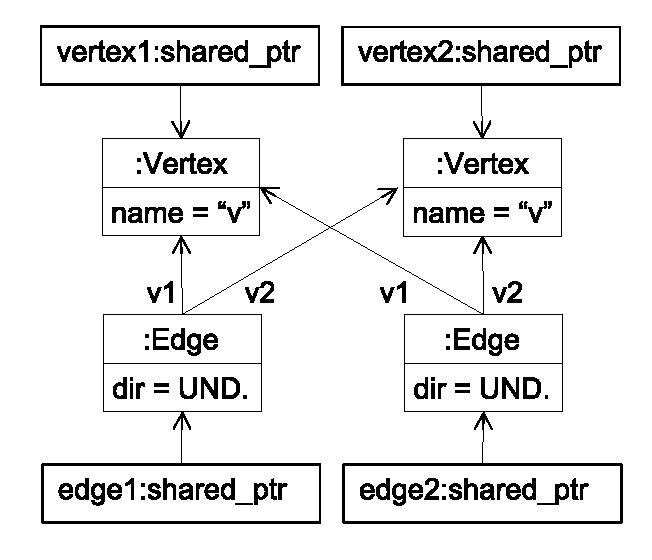
\includegraphics[width=.8\linewidth]{figs/vertices_edges_cpp.eps}
  \caption{Physical}
  \label{fig:vertices_edges-physical}
\end{subfigure}
\begin{subfigure}{.2\textwidth}
  \centering
  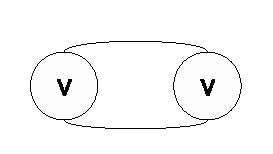
\includegraphics[width=.8\linewidth]{figs/vertices_edges_logical.eps}
  \caption{Logical}
  \label{fig:vertices_edges_logical}
\end{subfigure}
\caption{Vertices and edges: physical representation of the C++ objects and a traditional visual representation of the two vertices and edges}
\label{fig:vertices_edges}
\end{figure}

In uunet, vertices and edges may be included in a graph, where a graph:
\begin{itemize}
    \item guarantees ownership, that is, vertices and edges will keep existing at least until when they are inside some graph,
    \item allows to associate attributes to vertices and edges, that are local to the graph, and
    \item can create new vertices and edges.
\end{itemize}

\begin{figure}
    \centering
    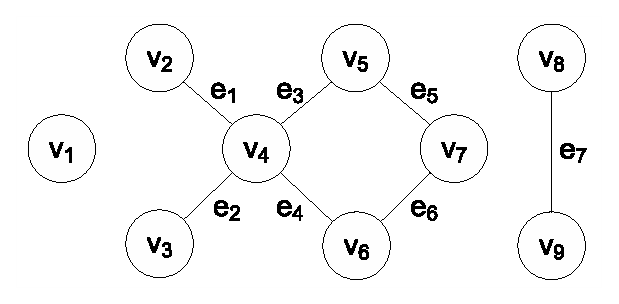
\includegraphics[width=.6\linewidth]{figs/G.eps}
    \caption{A simple graph $G$}
    \label{fig:G}
\end{figure}


To introduce basic concepts in graph theory, in this chapter we use the graph $G = (V, E)$ in Figure~\ref{fig:G}:
\begin{itemize}
    \item $ V = \{ v_1, v_2, v_3, v_4, v_5, v_6, v_7, v_8, v_9 \} $
    \item $ E = \{ e_1, e_2, e_3, e_4, e_5, e_6, e_7, e_8 \} $, where $ e_1 = (v_2, v_4)$, etc.
\end{itemize}

\begin{lstlisting}[style=c++]
// Reading the graph from file
#include "io/read_network.hpp"
const string network_file = "../simple.txt";
auto g = read_network(network_file, "G", ',');

// Vertices
auto v1 = g->vertices()->get("v1");
auto v2 = g->vertices()->get("v2");
auto v3 = g->vertices()->get("v3");
auto v4 = g->vertices()->get("v4");
auto v5 = g->vertices()->get("v5");
auto v6 = g->vertices()->get("v6");
auto v7 = g->vertices()->get("v7");
auto v8 = g->vertices()->get("v8");
auto v9 = g->vertices()->get("v9");

// Edges
auto e1 = g->edges()->get(v2, v4);
auto e2 = g->edges()->get(v3, v4);
auto e3 = g->edges()->get(v5, v4);
auto e4 = g->edges()->get(v6, v4);
auto e5 = g->edges()->get(v5, v7);
auto e6 = g->edges()->get(v6, v7);
auto e7 = g->edges()->get(v8, v9);
\end{lstlisting}

We say that:
\begin{itemize}
    \item $v_2$ and $v_4$ are \emph{end-vertices} of $e_1$.
    \item $v_2$ and $v_4$ are \emph{adjacent}.
    \item $v_2$ is a \emph{neighbor} of $v_4$, $v_4$ is a \emph{neighbor} of $v_2$.
    \item $e_1$ is \emph{incident} to $v_2$ and $v_4$.
\end{itemize}

In the following we show the corresponding code in \code{uunet}.
\begin{lstlisting}[style=c++] 
cout << "End-vertices of e1: "
    << e1->v1->name << ", " << e1->v2->name 
    << endl;
\end{lstlisting}
\begin{lstlisting}[style=out]
End-vertices of e1: v2, v4
\end{lstlisting}

\begin{lstlisting}[style=c++]
auto neigh = g->edges()->neighbors(v4);
cout << "Neighbors of v4: ";
for (auto v: *neigh)
{
    cout << v->name << " ";
}
cout << endl;
\end{lstlisting}
\begin{lstlisting}[style=out]
Neighbors of v4: v2 v3 v5 v6 
\end{lstlisting}

\begin{lstlisting}[style=c++] 
auto inc = g->edges()->incident(v4);
cout << "Edges incident to v4:" << endl;
for (auto e: *inc)
{
    cout << "(" << e1->v1->name << " -- " << e1->v2->name << ") ";
}
cout << endl;
\end{lstlisting}
\begin{lstlisting}[style=out]
Edges incident to v4:
(v2 -- v4) (v3 -- v4) (v4 -- v5) (v4 -- v6) 
\end{lstlisting}



%\section{Special types of graphs}

%Independent set: for every pair of vertices u, v ∈ V′, there is no edge in G joining the two vertices u and v.

%Bipartite graph. Partite sets.

%\section{Isomorphism}

%There is no known polynomial time algorithm to check if two graphs are isomorphic.

%\section{Walks, trails and paths}



\chapter{Networks} \label{ch:networks}

As we have seen in the previous chapter, \code{uunet} defines some basic types of network models, that are reviewed in more detail in Section \ref{ch:nets:basic}. Using cubes, more general custom models can be defined, as shown in Section \ref{ch:nets:cubes}.

\section{Predefined models} \label{ch:nets:basic}

\subsection{Basic networks}

The four main combinations defining the types of allowed edges are obtained by specifying edge directionality, and whether a network allows loops.

\begin{definition}[Loop]
A loop is an edge with the same end-vertices. 
\end{definition}

\begin{lstlisting}[style=c++]
auto dir = EdgeDir::UNDIRECTED;
auto und = EdgeDir::UNDIRECTED;
auto loops = LoopMode::ALLOWED;
auto no_loops = LoopMode::DISALLOWED;
\end{lstlisting}
    
The following example creates an undirected network not allowing loops (which is checked behind the scenes using an observer monitoring the insertion of new edges):
\begin{lstlisting}[style=c++]
auto g = make_unique<Network>("g", und, no_loops);
auto v1 = g->vertices()->add("v1"); // new vertex
auto v2 = g->vertices()->add("v2"); // new vertex
auto e = g->edges()->add(v1, v2); // new edge
g->edges()->contains(v2, v1); // true
// g->edges()->add(v1, v1); // throws exception
\end{lstlisting}
A network also allows to add attributes to its vertices and edges: the \code{attr} functions return pointers to \code{AttributeStore}s (see Section \ref{ch:core:attr} for the list of attribute handling functions provided by \code{AttributeStore}s):
\begin{lstlisting}[style=c++]
g->vertices()->attr();
g->edges()->attr();
\end{lstlisting}
The following examples create a directed network allowing loops:
\begin{lstlisting}[style=c++]
auto g2 = make_unique<Network>("g", dir, loops);
g2->vertices()->add(v1); // adding existing vertex v1
g2->vertices()->add(v2);
g2->edges()->add(v1, v2);
g2->edges()->add(v1, v2); // return nullptr
g2->edges()->contains(v2, v1); // false
g2->edges()->add(v1, v1);
\end{lstlisting}
In \code{uunet}, a Network only allows simple edges, while a MultiNetwork allows multiple edges. 
\begin{definition}[Multiple edge]
Multiple edges are edges with the same pair of end-vertices.
\end{definition}
Both Network and MultiNetwork may allow or not loops, as specified when they are created.
\begin{lstlisting}[style=c++]
auto simple = make_unique<Network>("g", dir, false);
auto multi = make_unique<MultiNetwork>("g", dir, true);
\end{lstlisting}
Notice that a \code{MultiNetwork} has a different interface: the function \code{edges()->get()} returns a container of edges, not a single edge.
\begin{lstlisting}[style=c++]
auto mg = make_unique<MultiNetwork>("g", dir, loops);
mg->vertices()->add(v1);
mg->vertices()->add(v2);
mg->edges()->add(v1, v2);
mg->edges()->add(v1, v2);
mg->edges()->get(v1, v2); // returns two edges
\end{lstlisting}

\subsection{Weights, times and probabilities}

Networks can be made weighted:
\begin{lstlisting}[style=c++]    
make_weighted(g.get());
is_weighted(g.get()); // true
set_weight(g.get(), e, 3.14);
get_weight(g.get(), e); // 3.14
\end{lstlisting}
By default, an edge whose weight has not been set will return weight 1.

Probabilistic networks are defined and manipulated similarly to weighted networks, with the difference that probabilities must be in the [0,1] range:
\begin{lstlisting}[style=c++]
make_probabilistic(g.get());
is_probabilistic(g.get()); // true
// set_prob(g.get(), e, -.3); // throws exception
// set_prob(g.get(), e, 1.14); // throws exception
set_prob(g.get(), e, .14);
get_prob(g.get(), e); // .14
\end{lstlisting}

In a temporal network, multiple timestamps can be associated to the same edge. For example, if we define the following times:
\begin{lstlisting}[style=c++]
auto t1 = uu::core::epoch_to_time(17438);
auto t2 = uu::core::epoch_to_time(17468);
\end{lstlisting}
We can then associate both of them to the same edge:
\begin{lstlisting}[style=c++]
make_temporal(g.get());
is_temporal(g.get()); // true
add_time(g.get(), e, t1);
add_time(g.get(), e, t2);
get_times(g.get(), e); // returns two times
\end{lstlisting}


\subsection{Multilayer networks}

In a multilayer network we can add multiple networks as layers:
\begin{lstlisting}[style=c++]
auto mnet = make_unique<MultilayerNetwork>("m");
auto l1 = mnet->layers()->add("l1", dir, loops);
auto l2 = mnet->layers()->add("l2", und, no_loops);
\end{lstlisting}

\code{l1} and \code{l2} are of type Network*, so we can use them as seen above. However, one should be careful when adding vertices to them if we want to have the same vertices in different layers:
\begin{lstlisting}[style=c++]
l1->vertices()->add(v1); // adding existing vertex v1
l2->vertices()->add(v1); // adding existing vertex v1
\end{lstlisting}
The command \code{l2->vertices()->add("v1")} would instead create and add a different vertex.

The set of distinct vertices in a multilayer network are called actors:
\begin{lstlisting}[style=c++]
mnet->actors(); // {v1}, only one actor so far
\end{lstlisting}

In addition, a multilayer network allows us to add interlayer edges. Before adding edges between two layers, we have to initialize that pair. The following example initializes the pair of layers \code{l1,l2}, specifying that interlayer edges between these layers are directed, and adds two directed edge between \code{v11} in layer \code{l1} and \code{v1} in layer \code{l2}.
\begin{lstlisting}[style=c++]
mnet->interlayer_edges()->init(l1, l2, dir); 
mnet->interlayer_edges()->add(v1, l1, v1, l2);
mnet->interlayer_edges()->add(v1, l2, v1, l1);
\end{lstlisting}


\section{Construction of custom network models}\label{ch:nets:cubes}

Using cubes we can build several types of networks combining cubes in different ways. 

\subsection{Simple graphs}

A simple graph has a set of vertices, a set of edges between those vertices, and edges are undirected and do not allow loops:
\begin{lstlisting}[style=c++]
auto V = make_unique<VCube>("V");
auto E = make_unique<ECube>("E", V.get(), V.get(), EdgeDir::UNDIRECTED, LoopMode::DISALLOWED);
\end{lstlisting}
Once we have created \code{V} and \code{E} we can add vertices and edges.
\begin{lstlisting}[style=c++]
auto v1 = V->add("v1");
auto v2 = V->add("v2");
auto v3 = V->add("v3");
auto e1 = E->add(v1, v3);
auto e2 = E->add(v2, v3);
\end{lstlisting}
Notice that while cubes allow us to assemble many types of data models, for some models it can be more intuitive to wrap the cubes inside a better-known and more specific interface. For example, we may want to define networks, and retrieve their vertices, or we may want to define multiplex networks, and retrieve their actors, or we may be interested in getting messages from a temporal text network. In these cases, we can define an interface and use cubes to implement it behind the scenes, so that a user does not need to know about them for basic structures and operations. As an example, we can wrap the two cubes above inside a \code{Network}:
\begin{lstlisting}[style=c++]
auto g = make_unique<Network>("G", move(V), move(E));
g->vertices() // VCube*
g->edges() // ECube*
g->vertices()->add("v4") // const Vertex*
// etc.
\end{lstlisting}
Even when we create a network from scratch, behind the scenes the network is implemented using cubes, but this knowledge is not needed to work with the network.
\begin{lstlisting}[style=c++]
auto g = make_unique<Network>("G");
auto v1 = g->vertices()->add("v1") 
auto v2 = g->vertices()->add("v2") 
auto e1 = g->edges()->add(v1, v2) 
// etc.
\end{lstlisting}



\subsection{Multiplex and multirelational networks}

A multiplex network can be defined in different ways, corresponding to the variations found in the literature. In general, a multiplex network has a set of actors and a set of edges of different types.
So we can just first create a graph (we'll call its vertices \code{A} instead of \code{V}, for Actors):
\begin{lstlisting}[style=c++]
auto A = make_unique<VCube>("A");
auto E = make_unique<ECube>("E", A.get(), A.get());
\end{lstlisting}
then we can transform it into a multiplex network just by structuring its edges into multiple cells, one for each type of edges:
\begin{lstlisting}[style=c++]
E->add_dimension("e-type", {"friend", "work"});
\end{lstlisting}

Now we can add actors and edges between actors. Notice that we can add edges to specific cells.
\begin{lstlisting}[style=c++]
auto alice = A->add("Alice");
auto bob = A->add("Bob");
auto mirka = A->add("Mirka");
E->cell({"friend"})->add(alice, bob);
E->cell({"work"})->add(alice, bob);
E->cell({"friend"})->add(alice, mirka);
\end{lstlisting}
It is worth noticing that with this design this multiplex network has \emph{two multiplex} edges (and not three, as we would have in a multigraph): one multiplex edge between Alice and Bob on \code{friend} and \code{work}, and one edge only on \code{friend}.

An alternative design is to use different cubes for the different types of edges:
\begin{lstlisting}[style=c++]
auto A = make_unique<VCube>("A");
auto E1 = make_unique<ECube>("fri.", A.get(), A.get());
auto E2 = make_unique<ECube>("work", A.get(), A.get());
\end{lstlisting}
In this case we would be able to add different edges among the same actors in different cubes.

Finally, we can build a generalized multiplex network with different actors depending on the edges. For example, we can structure the actors into two cells, one with all the actors (that we call \code{offline}) and one only for the actors with a Facebook account:
\begin{lstlisting}[style=c++]
auto A = make_unique<VCube>("A");
A->add_dimension("actor-type", {"facebook", "offline"});
\end{lstlisting}
In this way we can specify facebook edges that can only join actors with a facebook account. To do this, we can build virtual VCubes on individual cells (or more in general slices of the cubes):
\begin{lstlisting}[style=c++]
auto fb = vslice("facebook", A.get(), {{0}});
auto Efb = make_unique<ECube>("fb", fb.get(), fb.get());
\end{lstlisting}
Notice that \code{fb} is itself a VCube. In addition, the \code{vslice()} function does not replicate any vertex pointer, because it creates a single-cell cube that is a virtual view over the original one (as in SQL) and so it occupies a marginal amount of additional memory not depending on the size of the original cube.

\subsection{General multilayer networks}

Finally, we can add "interlayer" edges between actors of different types to obtain a general multilayer network:
\begin{lstlisting}[style=c++]
auto off = vslice("offline", A.get(), {{1}});
auto IE = make_unique<ECube>("ie", off.get(), fb.get());
auto e1 = IE->add(alice, off.get(), bob, fb.get());
auto e2 = IE->add(bob, off.get(), alice, fb.get());
auto e3 = IE->add(mirka, off.get(), bob, fb.get());
\end{lstlisting}


\subsection{Temporal interlayer edges}
\label{sec:discr}

Using the attribute handling functionality of the cubes we can extend the previous data models with times, weights, probabilities, text messages and other attributes. For some special attributes (times, weights and probabilities) that are very common and have specialized algorithms requiring them, we can also use utility functions to setup the cubes (e.g., making their elements temporal, or uncertain) and manipulate these special attributes. The following example extends our interlayer edges with temporal information, then adding one or more timestamps to each of them:
\begin{lstlisting}[style=c++]
make_temporal(IE);
add_time(IE.get(), e1, "1970-01-01 01:01:07+0000");
add_time(IE.get(), e1, "1970-01-02 07:21:07+0000");
add_time(IE.get(), e2, "1970-01-02 13:09:05+0000");
add_time(IE.get(), e3, "1970-01-03 14:01:07+0000");
\end{lstlisting}
Here we have specified times as strings with a standard format, but we can express them in different ways, using the library's own \code{Time} format, or the number of seconds from epoch or custom string representations of time.

If we want to slice the edges into multiple time windows we can use a discretization function, which is a fundamental concept in the theory of multilayer cubes and for practical applications. One can define custom discretization functions, but here we use a predefined one that takes a minimum time, a maximum time and the number of windows as input and if used while adding a (temporal) dimension it redistributes the original edges in the new cells. In the next example, three slices/layers are created:
\begin{lstlisting}[style=c++]
Time min = to_time("1970-01-01 00:00:00+0000");
Time max = to_time("1970-01-03 23:59:59+0000");
auto d = UniformTemporalDiscretization<ECube>(IE.get(), min, max, 3);
IE->add_dimension("times", {"day1", "day2", "day3"}, d);
\end{lstlisting}
Now the extended ECube \code{IE} still contains all the original edges (because all of them had at least one associated time between \code{min} and \code{max}), but if we access the individual cells we will find respectively edge \code{e1} (day1), edges \code{e1} and \code{e2} (day2), and edge \code{e3} (day3). The same functionality can be used to assign tweets to different topical layers based on their hashtags, actors to different institution layers based on their affiliations, etc.

    
\chapter{Creating networks} \label{ch:creation}

Networks can be created in multiple ways: manually, that is, individually adding vertices and edges as seen above, or calling functions which create standard types of graphs, or using input/output functions, or using network generation models. All these (apart from manual creation) are reviewed in this chapter.

\section{Standard graphs}

The following pre-defined graphs can be created. The corresponding networks are shown in Figure \ref{fig:notable}.
\begin{lstlisting}[style=c++] 
#include "generation/standard_graphs.hpp"
auto n_5 = null_graph(5);
auto p_5 = path_graph(5);
auto c_5 = cycle_graph(5);
auto w_5 = wheel_graph(5);
auto k_5 = complete_graph(5);
auto k_3_2 = complete_bipartite_graph(3, 2);
\end{lstlisting}

\begin{figure}
  \centering
\begin{subfigure}{.26\textwidth}
  \centering
  
\includegraphics[width=.8\linewidth]{figs/N5.eps}
  \caption{$N_5$}
  \label{fig:notable-N5}
\end{subfigure}
\begin{subfigure}{.26\textwidth}
  \centering
  
\includegraphics[width=.8\linewidth]{figs/P5.eps}
  \caption{$P_5$}
  \label{fig:notable-P5}
\end{subfigure}
\begin{subfigure}{.26\textwidth}
  \centering
  
\includegraphics[width=.8\linewidth]{figs/C5.eps}
  \caption{$C_5$}
  \label{fig:notable-C5}
\end{subfigure}
\newline
  \centering
\begin{subfigure}{.26\textwidth}
  \centering
  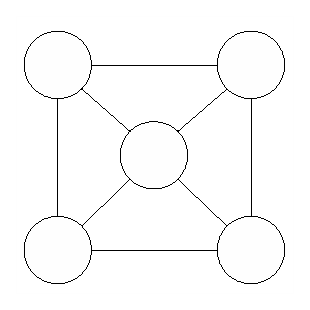
\includegraphics[width=.8\linewidth]{figs/W5.eps}
  \caption{$W_5$}
  \label{fig:notable-W5}
\end{subfigure}
\begin{subfigure}{.26\textwidth}
  \centering
  
\includegraphics[width=.8\linewidth]{figs/K5.eps}
  \caption{$K_5$}
  \label{fig:notable-K5}
\end{subfigure}
\begin{subfigure}{.26\textwidth}
  \centering
  
\includegraphics[width=.8\linewidth]{figs/K23.eps}
  \caption{$K_{2,3}$}
  \label{fig:notable-K23}
\end{subfigure}
\caption{Special graphs: null graph, path graph, cycle graph, wheel graph, complete graph, complete bipartite graph}
\label{fig:notable}
\end{figure}



\section{I/O}  \label{ch:io}

The general syntax to read a network from file is the following:

\begin{lstlisting}[style=file]
#VERSION           
2.0                
                   
#TYPE              
directed           
                   
#VERTEX ATTRIBUTES 
a1,string          
                   
#EDGE ATTRIBUTES   
a1,double          
                   
#VERTICES          
v1,a_value         
v2,another_value   
v4,one_more_value  
                   
#EDGES             
v1,v2,2.3          
v1,v3,4            
v2,v1,3            
v1,v4,4.2          
\end{lstlisting}
By default edges are undirected, so if no attributes are present the following is also a valid input file:
\begin{lstlisting}[style=file]
v1,v2              
v1,v3              
v1,v4              
\end{lstlisting}
Under \#TYPE we can also specify whether the network is weighted:
\begin{lstlisting}[style=file]  
#TYPE              
directed           
weighted    
\end{lstlisting}        
If the network is weighted, then the first attribute value for edges must be the weight:
\begin{lstlisting}[style=file]         
#EDGES             
v1,v2,143,2.3      
v1,v3,11,4         
v2,v1,14,3         
v1,v4,10,4.2       
\end{lstlisting}
    
Multilayer networks allow to specify the features of each layer, and also differentiate between actors and vertices:
\begin{lstlisting}[style=file]
#TYPE                
multilayer           
                     
#VERSION             
2.0                  
                     
#LAYERS              
l1,l1,UNDIRECTED     
l2,l2,UNDIRECTED,LOOPS
l1,l2,DIRECTED       
                     
#ACTOR ATTRIBUTES    
ssn, string          
                     
#ACTORS              
v1,122343242         
v3,122343654         
                     
#VERTEX ATTRIBUTES   
l2,day,string        
                     
#VERTICES            
v6,l2,Monday         
                     
#EDGE ATTRIBUTES     
l1,attr1,numeric 
attr2,numeric   
                     
#EDGES               
v1,l1,v2,l1,1,7      
v1,l1,v5,l1,2,8      
v2,l1,v5,l1,3,9      
v2,l1,v3,l1,4,10     
v2,l1,v4,l1,5,11     
v3,l1,v4,l1,6,12     
v1,l1,v4,l2,13       
v2,l1,v3,l2,14       
v2,l1,v4,l2,15       
v3,l1,v3,l2,16       
v3,l1,v4,l2,17       
v1,l1,v2,l2,18       
\end{lstlisting}
In the example above, attr1 is an attribute of edges in layer 1, while attr2 is a global attribute.


Edges in a multiplex network are instead expressed only specifying the layer once, as interlayer edges are not allowed:

\begin{lstlisting}[style=file]              
l1,v1,v2,1,7      
l1,v1,v5,2,8  
\end{lstlisting}

\emph{Note: after the introduction of cubes we may define a new input format that allows more flexibility, without breaking backward compatibility. Working on it.}

\section{Generation}  \label{ch:generation}

Three types of network generation approaches are currently available. ER models for simple graphs, multilayer network co-evolution, and multilayer community-based.

\subsection{Simple graphs}

ER graphs can be created using either the np model, specifying the number of vertices and the probability for every pair of vertices of being adjacent, or the nm model, specifying the number of vertices and the number of edges:
\begin{lstlisting}[style=c++]
auto er_np = erdos_renyi_np(10, .2);
auto er_nm = erdos_renyi_nm(10, 4); 
\end{lstlisting}

\subsection{Multilayer network coevolution}

Multilayer networks can be generated using a co-evolutionary model where, for every layer, we specify the probability that the layer evolves according to internal dynamics or importing an edge from another layer. A dependency matrix is used to specify from which other layers the edge can be imported, and with which probability.
\begin{lstlisting}[style=c++]
vector<string> layer_names = {"l1", "l2"};
vector<double> pr_internal_event = {.8, .5};
vector<double> pr_external_event = {0, .5};
vector<vector<double>> dependency = {{0, 1}, {1, 0}};
\end{lstlisting}
The internal evolution dynamic is specified in the form of an evolution model, either connecting vertices uniformly at random (\code{ERModel}) or using preferential attachment (\code{PAModel}).
\begin{lstlisting}[style=c++]
vector<EvolutionModel<MultilayerNetwork>*> ev_model;
auto pa = make_unique<PAModel<MultilayerNetwork>>(3, 2);
auto er = make_unique<ERModel<MultilayerNetwork>>(50);
ev_model.push_back(pa.get());
ev_model.push_back(er.get());
\end{lstlisting}
Finally, we have to specify how many evolution steps we want to run:
\begin{lstlisting}[style=c++]
size_t num_of_steps = 100;
\end{lstlisting}
    
The function \code{evolve} takes all these parameters and lets the multilayer network grow. Assume that \code{ml} is a pointer to a multilayer network with two layers.
\begin{lstlisting}[style=c++]
evolve(ml, layer_names,
       pr_internal_event, pr_external_event, 
       dependency, ev_model,
       num_of_steps);
\end{lstlisting}

\subsection{Community-based}

The last way to obtain a multilayer network is by passing a pointer to a community structure as input (see Chapter \ref{ch:community}) specifying the the probability for two vertices of being adjacent if they are inside the same community or in different communities, for each layer. 
\begin{lstlisting}[style=c++]
sample(ml, com, {.5, .5}, {.01, .01});
\end{lstlisting}

\chapter{Operations} \label{ch:operations}

The \code{operations/} module contains functions to manipulate networks.
    
\section{Simple graph operations}

The library supports basic operations from graph theory.

\subsection{Graph induction}

A first type of operations is graph induction. The definitions and corresponding library functions follow. Notice that the following functions return unique pointers to \code{Network}s.

\begin{definition}[Vertex-induced subgraph]
Let $G = (V, E)$ and $V' \subseteq V$. The vertex-induced subgraph $G_{|V'} = (V', E')$ where $ E' = \{ (u,v) \ | \ u, v  \in V' \}$.
\end{definition}

\begin{lstlisting}[style=c++]
std::vector<const Vertex*> vs1 = {v2, v4, v5};
auto g_sub1 = vertex_induced_subgraph(g.get(), 
                        vs1.begin(), vs1.end());
    
std::vector<const Vertex*> vs2 = {v4, v5, v6};
auto g_sub2 = vertex_induced_subgraph(g.get(), 
                        vs2.begin(), vs2.end());
\end{lstlisting}

\begin{definition}[Edge-induced subgraph]
Let $G = (V, E)$ and $E' \subseteq E$. The vertex-induced subgraph $G_{|E'} = (V', E')$ where $ V' = \{ v \ | \ e  \in E' \land v \mbox{ is an end-vertex of } e \}$.
\end{definition}

Edge-induced subgraphs can be obtained using the function \code{edge\_induced\_subgraph()}.

\subsection{Vertex-set operations}

A second type of operations is set-based manipulation. The definitions and corresponding library functions follow.

\begin{definition}[Union]
Let $G_1 = (V1, E1)$ and $G_2 = (V2, E2)$ be two graphs. Then $G_1 \cup G_2 = (V1 \cup V2, E1 \cup E2)$
\end{definition}

Please notice that according to this definition and in a setting where edges have identities, in general the union of two simple graphs can be a multigraph.

\begin{lstlisting}[style=c++]
graph_union(g_sub1.get(), g_sub2.get());
\end{lstlisting}

\begin{definition}[Intersection]
Let $G_1 = (V1, E1)$ and $G_2 = (V2, E2)$ be two graphs. Then $G_1 \cap G_2 = (V1 \cap V2, E1 \cap E2)$
\end{definition}

\begin{lstlisting}[style=c++]
graph_intersection(g_sub1.get(), g_sub2.get());
\end{lstlisting}

\begin{definition}[Complement]
Let $G = (V, E)$. Then $\overline{G} = (V, E')$ where $ E' = \{ (u,v) \ | \ u, v  \in V \land (u,v) \notin E \}$.
\end{definition}

This definition adapts to the type of graph: it is appropriate for digraphs and also in case of loops.

\begin{lstlisting}[style=c++]
graph_complement(g_sub1.get());
\end{lstlisting}

\subsection{Edge operations}

A third type of operations manipulate edges. We can divide an edge, adding a new vertex in between:

\begin{lstlisting}[style=c++]
auto v10 = edge_subdivision(g.get(), e7, "v10");
auto e8 = g->edges()->get(v8, v10);
auto e9 = g->edges()->get(v10, v9);
\end{lstlisting}

And we can replace an edge with a new vertex:    
\begin{lstlisting}[style=c++]
edge_contraction(g.get(), e9, "v11");
\end{lstlisting}
    
\section{Flattening and projection}

Flattening adds the edges from a number of layers to a target network/layer. For example, assume that \code{net} contains two layers, \code{l1} and \code{l2}. We can add a new layer \code{lf1} and add all edges in either \code{l1} or \code{l2} to it as follows:
\begin{lstlisting}[style=c++]
auto l = {l1, l2};
auto lf1 = net->layers()->add("flat");
flatten_unweighted(l.begin(), l.end(), lf1);
\end{lstlisting}
    
Notice that the target network does not need to be a layer in the input multilayer network: we can flatten the layers into a layer in another multilayer network, or create a separate (simple) network that is the flattening of the input one.

In addition, we can use a weighted flattening so that a weight is added to each edge in the flattened network, indicating in how many original layers the edge was present.
\begin{lstlisting}[style=c++]
auto lf2 = net->layers()->add("w_flat");
flatten_weighted(l.begin(), l.end(), lf2);
\end{lstlisting}

While a flattening works on multiple networks, if a multilayer network has interlayer edges we can also compute a projection. In the following example two vertices in layer \code{l1} will be adjacent in the target layer/network \code{lf} whenever the two vertices are adjacent to a common vertex in \code{l2}.
\begin{lstlisting}[style=c++]
auto lf = net->layers()->add("flat");
project_unweighted(net.get(), l2, l1, lf);
\end{lstlisting}
    

\section{Anonymization}

TBD

\chapter{Measures} \label{ch:measures}

\section{Degree-based measures}

\subsection{Degree}

\begin{definition}[Degree]
The degree of a vertex $v$ in a graph $G$, notated $\mathrm{deg}(v)$, is the number of edges incident to $v$ in $G$\footnote{Loops are counted twice.}. 
\end{definition}

In \code{uunet} we have the following degree-based functions.

\begin{lstlisting}[style=c++] 
for (auto v: *g->vertices())
{
    size_t deg = degree(g.get(), v);
    cout << "deg(" << (*v) << "): "
        << deg << endl;
}
\end{lstlisting}
\begin{lstlisting}[style=out]
deg(v2): 1
deg(v1): 0
deg(v3): 1
deg(v5): 2
deg(v6): 2
deg(v7): 2
deg(v8): 1
deg(v9): 1
deg(v4): 4
\end{lstlisting}


\begin{lstlisting}[style=c++] 
auto avg_deg = average_degree(g.get());
cout << "Average degree: " << avg_deg << endl;
\end{lstlisting}
\begin{lstlisting}[style=out]
Average degree: 1.55556
\end{lstlisting}

With loops, there exists at least a graph for any degree sequence whose sum is even. Without loops, there are some degree sequences that cannot correspond to any graph.

\begin{lstlisting}[style=c++] 
cout << "Degree sequence: ";
auto deg_seq = degree_sequence(g.get());
for (auto deg: deg_seq)
{
    cout << deg << " ";
}
cout << endl;
\end{lstlisting}
\begin{lstlisting}[style=out]
Degree sequence: 0 1 1 1 1 2 2 2 4 
\end{lstlisting}
    
\begin{lstlisting}[style=c++] 
cout << "Degree distribution: ";
auto deg_distr = degree_distribution(g.get());
for (auto freq: deg_distr)
{
    cout << freq << " ";
}
cout << endl;
\end{lstlisting}
\begin{lstlisting}[style=out]
Degree distribution: 1 4 3 0 1 
\end{lstlisting}

For weighted networks we can also compute the strength of a vertex, that is the sum of the weights in its incident edges (loops being counted twice):
\begin{lstlisting}[style=c++]
strength(g.get(), v1);
\end{lstlisting}

For probabilistic networks we can also compute the expected degree of a vertex:
\begin{lstlisting}[style=c++]
exp_degree(g.get(), v1);
\end{lstlisting}

\subsection{Multilayer degree}

Degree in multilayer networks is computed in the same way as in single networks, where the degrees of an actor in all the input layers are added together:
\begin{lstlisting}[style=c++] 
auto l = net->layers();
size_t degree = degree(l.begin(), l.end(), v2);
\end{lstlisting}

The degree deviation of a vertex is just the standard deviation of its degree on the input layers:
\begin{lstlisting}[style=c++] 
double dd = degree_deviation(l.begin(), l.end(), v2);
\end{lstlisting}

\subsection{Neighborhood}

The multilayer degree function counts the same neighbor multiple times if it is a neighbor in more than one layer. Instead, we can extract the distinct neighbors of an actor, that are the actors adjacent to it in any of the input layers:
\begin{lstlisting}[style=c++] 
neighbors(net->layers()->begin(), net->layers()->end(), v1);
\end{lstlisting}

Exclusive neighbors are instead those which are neighbors in the input layers but not in the other layers in the network. Notice that in this case we also have to pass a pointer to the multilayer network.
\begin{lstlisting}[style=c++] 
vector<const Network*> l = {l1};
xneighbors(net.get(), l.begin(), l.end(), v2);
\end{lstlisting}

\section{Path-based}

\subsection{Distances}

The distance between two vertices can be computed on single and multilayer networks. For single networks the library implements Dijkstra's algorithm (available under \code{algorithms/}):
\begin{lstlisting}[style=c++] 
single_source_path_length(g, v2)
\end{lstlisting}

While for multilayer networks we can compute a generalized pareto distance:
\begin{lstlisting}[style=c++] 
pareto_distance(net.get(), v1);
\end{lstlisting}

%$w : E \rightarrow \mathcal{R}$

%For a walk $W = (e_1, \dots, e_n)$, the length of $W$ is $w(W) = w(e_1) + \dots + w(e_n)$.

%Distance:
%\[
%    d(u, v) = 
%    \left\{
%    \begin{array}{ll}
%        \infty & \text{no path from u to v}\\
%        \min\{w(W) : \text{W is a path from u to v}\} & \text{otherwise}\\
%    \end{array}
%    \right.
%\]

%Note: paths are used in case of negative weights.
    
\subsection{Betweenness}

Betweenness is currently implemented for single networks:
\begin{lstlisting}[style=c++]
auto C_b = betweenness(g.get());
C_b[v4]; // Betweenness of vertex v4
\end{lstlisting}

\section{Layer relevance}

The fraction of an actor's neighbors that are present in a subset of the layers is called layer relevance for the actor, and is computed as follows:
\begin{lstlisting}[style=c++]
vector<const Network*> l = {l1};
relevance(net.get(), l.begin(), l.end(), v1);
\end{lstlisting}

The fraction of an actor's neighbors that are present in a subset of the layers but not in the others is called exclusive layer relevance, and is computed as follows:
\begin{lstlisting}[style=c++]
vector<const Network*> l = {l1};
xrelevance(net.get(), l.begin(), l.end(), v1);
\end{lstlisting}

\section{Layer comparison}

Using property matrices we can define several functions to compare layers. Two that are pre-packaged into individual functions are Jaccard Edge and Pearson Degree, computing respectively the Jaccard coefficient of edges in the two layers and the Pearson correlation coefficient computed on the degrees of the actors in the two layers.
\begin{lstlisting}[style=c++]
jaccard_edge(net.get(), l1, l2);

pearson_degree(net.get(), l1, l2);
\end{lstlisting}


\chapter{Community detection} \label{ch:community}

The \code{community/} module provides data structures to represent communities, community detection algorithms, and evaluation functions.
Functions to read and write communities from/to file are in \code{io/}. 

\section{Data structures}

A Community Structure is a set of communities, and a Community is a set of elements. Communities are represented using a template class so that the type of elements adapts to the type of network. For example, in a community over networks its elements are vertices:
\begin{lstlisting}[style=c++]
auto com = make_unique<CommunityStructure<Network>>();

auto c1 = make_unique<Community<Network>>();
auto c2 = make_unique<Community<Network>>();

auto v1 = make_unique<Vertex>("v1");
auto v2 = make_unique<Vertex>("v2");

// Adding vertices to the community

c1->add(v1.get());
c1->add(v2.get());
c2->add(v2.get());

// Adding communities to the community structure

com->add(move(c1));
com->add(move(c2));
\end{lstlisting}

A community over a multilayer network has multilayer vertices as elements:
\begin{lstlisting}[style=c++]
auto ml_c = make_unique<Community<MultilayerNetwork>>();

// Creating multilayer vertices

auto n = make_unique<Network>("net");
auto ml_v1 = MLVertex(v1.get(), n.get());
auto ml_v2 = MLVertex(v2.get(), n.get());

// Adding multilayer vertices to the community

ml_c->add(ml_v1);
ml_c->add(ml_v2);
\end{lstlisting}

In general, one does not manually create communities, but obtains them using community detection algorithms.

\section{Algorithms}

The library provides two community detection algorithms for single networks:
\begin{lstlisting}[style=c++]
auto comm1 = label_propagation(net.get());
auto comm2 = louvain(net.get());
\end{lstlisting}
    and five algorithms for multilayer networks.
\begin{lstlisting}[style=c++]
auto mlcomm1 = mlcpm(mlnet.get(), 3, 1);
auto mlcomm2 = abacus(mlnet.get(), 3, 1);
auto mlcomm3 = glouvain2(mlnet.get(), 1.0);
auto mlcomm4 = infomap(mlnet.get());
auto mlcomm5 = mlp(mlnet.get());
\end{lstlisting}
    
\section{Evaluation}

Two community structures can be compared using normalized mutual information (for partitioning communities) and omega index (for overlapping communities):
\begin{lstlisting}[style=c++]
nmi(comm1.get(), comm2.get(), order(net.get()));
omega_index(comm1.get(), comm2.get(), order(net.get()));
\end{lstlisting}

The library also provides a function to compute multilayer modularity:
\begin{lstlisting}[style=c++]
modularity(mlnet.get(), mlcomm3.get(), 1.0);
\end{lstlisting}

\section{I/O} \label{ch:community:io}

If one needs to compare communities found by an algorithm against some ground truth, then it can be useful to read communities from a file. The format for multilayer communities requires the name of the actor, the name of the layer and the community id, starting from $0$.

\begin{lstlisting}[style=file]
vertex_name1,layer_name1,0
vertex_name2,layer_name1,0
% etc.
vertex_name1,layer_name2,1
% etc.
\end{lstlisting}

The \code{io/} module provides functions to read and write community files. Notice that the second parameter of the reading function is a multilayer network, so that the names of actors and layers can be matched with those in the network.
\begin{lstlisting}[style=c++]
read_multilayer_communities("com.txt", ml_net.get());

write_multilayer_communities(communities.get(), fname);
\end{lstlisting}
The \code{read\_multilayer\_communities()} function returns a unique pointer to a community structure.

\chapter{Layout}

The library does not provide functions to draw network diagrams. Some basic functions to do so are available in the R and Python versions.

However, two functions are available in the \code{layout/} module to compute coordinates. The first, \code{multiforce}, is a force-based layout computing coordinates inside a frame width $\times$ length. The parameters are the intralayer forces (repelling different vertices, and attracting adjacent ones), the interlayer forces (aligning the same actor on different layers) and gravity (attracting vertices towards the center of the frame). The last parameter is the number of iterations.
\begin{lstlisting}[style=c++]
multiforce(net, 10, 10, 
           w_intra, w_inter, gravity,
           100
);
\end{lstlisting}

A circular layout draw all the vertices in a circle of radius r:
\begin{lstlisting}[style=c++]
circular(net, r);
\end{lstlisting}

\chapter{Further readings} \label{ch:readings}

In addition to our book, we have written an article explaining how to use the R version of the library:
\begin{quote}
Matteo Magnani, Luca Rossi and Davide Vega. Multiplex network analysis with R. Journal of Statistical Software. (forthcoming) 
\end{quote}
and various articles summarizing the state of the art on specific aspects of multilayer network analysis (at the time of writing), including overviews about community detection: 
\begin{quote}
Matteo Magnani, Obaida Hanteer, Roberto Interdonato, Luca Rossi and Andrea Tagarelli. Community Detection in Multiplex Networks. ACM Computing Surveys (forthcoming) 
\end{quote}
pre-processing:
\begin{quote}
Roberto Interdonato, Matteo Magnani, Diego Perna, Andrea Tagarelli and Davide Vega. Multilayer network simplification: approaches, models and methods. Computer Science Review, 36, Elsevier.
\end{quote}
layer comparison:
\begin{quote}
Piotr Brodka, Anna Chmiel, Matteo Magnani and Giancarlo Ragozini (2018). Quantifying layer similarity in multiplex networks: a systematic study. Royal Society Open Science, 5(8). 
\end{quote}
and diffusion/propagation:
\begin{quote}
Mostafa Salehi, Rajesh Sharma, Moreno Marzolla, Matteo Magnani, Payam Siyari, and Danilo Montesi (2015). Spreading Processes in Multilayer Networks. IEEE Transactions on Network Science and Engineering 2 (2): 65--83.
\end{quote}

The following survey papers on general multilayer networks can also be of interest as they provide broad overviews of the research on multilayer networks from different perspectives: 

\begin{quote}
Mikko Kivel\"a, Alexandre Arenas, Marc Barthelemy, James P. Gleeson, Yamir Moreno, and Mason A. Porter. 2014. Multilayer Networks. Physics and Society. Journal of Complex Networks 2 (3): 203--71. 
\end{quote}

\begin{quote}
Stefano Boccaletti, Ginestra Bianconi, Regino Criado, Charo I. Del Genio, Jes\'us G\'omez-Garde\~nes, Miguel Romance, Irene Sendi\~na-Nadal, Zhen Wang, and Massimiliano Zanin. 2014. The Structure and Dynamics of Multilayer Networks. Physics Reports 544 (1): 1--122.
\end{quote}

%	\include{multiToC}

    %\appendix
    %\cleardoublepage\part{Appendix}
    %\chapter{Appendix Chapter}
    
\end{document}